\ifdefined\inMainDoc\else
\documentclass[12pt,a4paper]{article}
% ================================================================
%  PRÉAMBULE COMMUN - ANNALES CORRIGÉES
%  Université de Kara - FaST - Licence Fondamentale MPC
%  Design optimisé impression noir et blanc
% ================================================================

% -- ENCODAGE & LANGUE --
\usepackage[utf8]{inputenc}
\usepackage[T1]{fontenc}
\usepackage[french]{babel}
\usepackage{lmodern}
\usepackage{microtype}

% -- MISE EN PAGE --
\usepackage[a4paper, top=2.8cm, bottom=2.5cm, left=2.5cm, right=2.5cm, headheight=14pt]{geometry}
\usepackage{setspace}
\setstretch{1.2}
\usepackage{parskip}
\setlength{\parindent}{1.2em}
\setlength{\parskip}{4pt}

% -- MATHS --
\usepackage{amsmath, amssymb, mathtools, amsthm}
\usepackage{mathrsfs}
\usepackage{dsfont}
\usepackage{bm}
\usepackage{cancel}
\usepackage{textcomp}
% Définition de \oiint (intégrale de surface fermée) sans package supplémentaire
\newcommand{\oiint}{\mathop{\iint\!\!\!\!\!\!\!\bigcirc}\limits}

% -- PHYSIQUE & CHIMIE --
\usepackage{physics}
\usepackage{siunitx}
% Lorsque physics est chargé, siunitx omet \qty. On le restaure ici :
\AtBeginDocument{\RenewCommandCopy\qty\SI}
\sisetup{locale = FR, detect-all, output-decimal-marker={,}}
% Commande de substitution pour les unités posant problème avec pdflatex
% (ohm, degreeCelsius, micro, angstrom, percent utilisent des caractères non-ASCII)
\newcommand{\qtyohm}[1]{\ensuremath{\num{#1}\,\Omega}}
\newcommand{\qtydegc}[1]{\ensuremath{\num{#1}\,{}^\circ\text{C}}}
\newcommand{\qtyangstrom}[1]{\ensuremath{\num{#1}\,\text{\AA}}}
\newcommand{\qtypercent}[1]{\ensuremath{\num{#1}\,\%}}
\newcommand{\qtyum}[1]{\ensuremath{\num{#1}\,\mu\text{m}}}
\usepackage[version=4]{mhchem}

% -- GRAPHISMES --
\usepackage{graphicx}
\usepackage{float}
\usepackage{caption}
\usepackage{subcaption}
\usepackage{wrapfig}
\usepackage{tikz}
\usetikzlibrary{calc, arrows.meta, patterns, shapes.geometric}
\usepackage{pgfplots}
\pgfplotsset{compat=1.18}

% -- TABLEAUX --
\usepackage{booktabs}
\usepackage{array}
\usepackage{tabularx}
\usepackage{multirow}

% -- LISTES --
\usepackage{enumitem}
\setlist[enumerate]{topsep=3pt, itemsep=2pt, parsep=0pt}
\setlist[itemize]{topsep=3pt, itemsep=2pt, parsep=0pt, label={.}}

% -- BOÎTES (noir et blanc) --
\usepackage{mdframed}
\usepackage{tcolorbox}
\tcbuselibrary{skins, breakable, theorems}

% Boîte EXERCICE : encadré avec filet épais, fond blanc
\newmdenv[
  linewidth=1.2pt,
  linecolor=black,
  roundcorner=3pt,
  skipabove=10pt,
  skipbelow=6pt,
  innertopmargin=8pt,
  innerbottommargin=8pt,
  innerleftmargin=10pt,
  innerrightmargin=10pt,
  backgroundcolor=white,
  frametitle={\bfseries\small Exercice},
  frametitlealignment=\raggedright,
  frametitleaboveskip=4pt,
  frametitlebelowskip=4pt,
]{boiteexercice}

% Boîte CORRIGÉ : fond gris très clair + filet fin
\newmdenv[
  linewidth=0.6pt,
  linecolor=black,
  leftline=true,
  rightline=false,
  topline=false,
  bottomline=false,
  linecolor=black,
  innerleftmargin=12pt,
  innerrightmargin=8pt,
  innertopmargin=6pt,
  innerbottommargin=6pt,
  backgroundcolor=gray!8,
  skipabove=4pt,
  skipbelow=8pt,
]{boitecorrige}

% Boîte RÉSUMÉ DE COURS : double encadré
\newmdenv[
  linewidth=0.8pt,
  linecolor=black,
  roundcorner=2pt,
  backgroundcolor=gray!12,
  innertopmargin=10pt,
  innerbottommargin=10pt,
  innerleftmargin=12pt,
  innerrightmargin=12pt,
  skipabove=12pt,
  skipbelow=8pt,
]{boiteresume}

% Boîte ATTENTION/REMARQUE : barre gauche épaisse
\newmdenv[
  leftline=true,
  rightline=false,
  topline=false,
  bottomline=false,
  linewidth=3pt,
  linecolor=black,
  backgroundcolor=gray!5,
  innerleftmargin=12pt,
  innerrightmargin=8pt,
  innertopmargin=5pt,
  innerbottommargin=5pt,
  skipabove=6pt,
  skipbelow=6pt,
]{boiteremarque}

% -- DIFFICULTÉ DES EXERCICES --
\newcommand{\facile}{$\star$}
\newcommand{\moyen}{$\star\!\star$}
\newcommand{\difficile}{$\star\!\star\!\star$}
\newcommand{\niveau}[1]{\hfill\textbf{#1}\hspace{2pt}}

% -- EN-TÊTES ET PIEDS DE PAGE --
\usepackage{fancyhdr}
\pagestyle{fancy}
\fancyhf{}
\renewcommand{\headrulewidth}{0.5pt}
\renewcommand{\footrulewidth}{0.3pt}

% -- HYPERLIENS --
\usepackage[hidelinks]{hyperref}
\hypersetup{
    colorlinks=false,
    pdftitle={Annale Corrigée - Licence MPC - Université de Kara}
}

% -- TITRES --
\usepackage{titlesec}
\titleformat{\section}{\Large\bfseries}{\thesection.}{0.8em}{}[\vspace{2pt}\hrule\vspace{4pt}]
\titleformat{\subsection}{\large\bfseries}{\thesubsection.}{0.7em}{}
\titleformat{\subsubsection}{\normalsize\bfseries}{\thesubsubsection.}{0.6em}{}

% -- THÉORÈMES --
\theoremstyle{definition}
\newtheorem{defn}{Définition}[section]
\newtheorem{prop}{Propriété}[section]
\newtheorem{thm}{Théorème}[section]
\newtheorem{corol}{Corollaire}[section]
\newtheorem{exemple}{Exemple}[section]

% -- COMMANDES MATHÉMATIQUES UTILES --
\newcommand{\vect}[1]{\overrightarrow{#1}}
\newcommand{\R}{\mathbb{R}}
\newcommand{\N}{\mathbb{N}}
\newcommand{\Z}{\mathbb{Z}}
\newcommand{\C}{\mathbb{C}}
\renewcommand{\d}{\mathrm{d}}
\newcommand{\deriv}[2]{\dfrac{\d #1}{\d #2}}
\newcommand{\dpart}[2]{\dfrac{\partial #1}{\partial #2}}
\newcommand{\rot}{\overrightarrow{\mathrm{rot}}\,}
\renewcommand{\div}{\mathrm{div}\,}
\renewcommand{\grad}{\overrightarrow{\mathrm{grad}}\,}
\newcommand{\e}{\mathrm{e}}
\newcommand{\ii}{\mathrm{i}}
\renewcommand{\Tr}{\mathrm{Tr}}

% Numérotation des équations par section
\numberwithin{equation}{section}

% -- RÉSULTATS ENCADRÉS --
\newcommand{\res}[1]{\[\boxed{#1}\]}

% -- REMARQUE INLINE --
\newcommand{\rmq}[1]{\begin{boiteremarque}\textbf{Remarque.} #1\end{boiteremarque}}

% -- MISE EN VALEUR DU RÉSULTAT FINAL --
\newcommand{\reponse}[1]{%
  \begin{center}
    \fbox{\begin{minipage}{0.92\textwidth}\centering #1\end{minipage}}
  \end{center}%
}


\lhead{\small\textit{Mécanique Analytique - Licence 3}}
\rhead{\small\textit{FaST, Université de Kara}}
\cfoot{\thepage}

\begin{document}
\fi

\begin{center}
  {\LARGE\bfseries MÉCANIQUE ANALYTIQUE}\\[0.3cm]
  {\normalsize Licence 3 - Physique}\\[0.1cm]
  \rule{0.7\textwidth}{0.8pt}
\end{center}

\vspace{0.3cm}

\section*{Résumé du cours}

\begin{boiteresume}

\textbf{1. Principe de Hamilton.} Le mouvement réel d'un système entre deux instants $t_1$ et $t_2$ est celui qui rend stationnaire l'action $S = \int_{t_1}^{t_2} \mathcal{L}\,\d t$, où $\mathcal{L} = T - V$ est le lagrangien. Cela conduit aux équations d'Euler-Lagrange.

\textbf{2. Équations de Lagrange.} Pour un système à $n$ degrés de liberté de coordonnées généralisées $\{q_k\}$ :
\[
  \frac{\d}{\d t}\!\left(\frac{\partial \mathcal{L}}{\partial \dot{q}_k}\right) - \frac{\partial \mathcal{L}}{\partial q_k} = Q_k^{\mathrm{nc}}, \qquad k = 1,\ldots,n
\]
où $Q_k^{\mathrm{nc}}$ désigne les forces généralisées non conservatives (frottement, excitation externe). En l'absence de telles forces, $Q_k^{\mathrm{nc}} = 0$.

\textbf{3. Coordonnées généralisées et énergie cinétique.} On choisit un jeu de coordonnées $q_k$ adapté aux contraintes. L'énergie cinétique s'exprime sous la forme quadratique $T = \frac{1}{2}\sum_{i,j} M_{ij}(q)\,\dot{q}_i\dot{q}_j$.

\textbf{4. Intégrales premières.} Si $\mathcal{L}$ ne dépend pas explicitement du temps, l'énergie mécanique $E = T + V$ est conservée. Si $\mathcal{L}$ ne dépend pas d'une coordonnée $q_k$ (coordonnée cyclique), le moment généralisé conjugué $p_k = \partial\mathcal{L}/\partial\dot{q}_k$ est conservé.

\textbf{5. Hamiltonien et équations de Hamilton.} Le hamiltonien est défini par la transformée de Legendre :
\[
  \mathcal{H}(q_k, p_k, t) = \sum_k p_k\dot{q}_k - \mathcal{L}
\]
Les équations canoniques sont :
\[
  \dot{q}_k = \frac{\partial\mathcal{H}}{\partial p_k}, \qquad \dot{p}_k = -\frac{\partial\mathcal{H}}{\partial q_k}
\]
Si $\mathcal{H}$ ne dépend pas explicitement du temps, il est une intégrale première du mouvement.

\textbf{6. Crochets de Poisson.} Pour deux observables $f$ et $g$ :
\[
  \{f, g\} = \sum_k\left(\frac{\partial f}{\partial q_k}\frac{\partial g}{\partial p_k} - \frac{\partial f}{\partial p_k}\frac{\partial g}{\partial q_k}\right)
\]
Une observable $f$ est une intégrale première si et seulement si $\{\mathcal{H}, f\} = 0$ (et $\partial f/\partial t = 0$).

\end{boiteresume}

\newpage

\section{Déplacements virtuels et principe de d'Alembert}

\subsection*{Exercice 1 - Système de treillis articulé \niveau{\moyen}}

\begin{boiteexercice}
\begin{enumerate}
  \item Rappeler ce qu'est un déplacement virtuel et qu'appelle-t-on travail virtuel. Que devient ce travail si le système est statique ou se déplace à vitesse uniforme ?

  \item On considère une masse $m$ placée en $A$ et reliée par deux tiges rigides aux points $O$ et $B$. Les barres de longueur $OA = AB = l$ sont articulées en $A$. Le support de l'articulation $O$ est fixe et le patin articulé en $B$ peut glisser sans frottement le long de l'axe horizontal. Les articulations sont supposées parfaites et les masses des tiges et du patin sont négligeables.
  \begin{enumerate}
    \item[a)] Quel est le nombre de degrés de liberté de ce système ?
    \item[b)] En appliquant le principe de d'Alembert, quelle force $F$ faut-il appliquer au patin pour que le système reste en équilibre ?
    \item[c)] Déterminer la valeur de la réaction en $B$.
  \end{enumerate}
\end{enumerate}
\end{boiteexercice}

\begin{boitecorrige}
\begin{enumerate}
  \item Un déplacement virtuel est un déplacement infinitésimal imaginaire compatible avec les contraintes, effectué à un instant figé. Le travail virtuel est le travail de l'ensemble des forces actives lors de ce déplacement. Pour un système statique ou en mouvement uniforme, la résultante des forces extérieures est nulle, de sorte que le travail virtuel de toutes les forces est nul.

  \item La masse $m$ se déplace dans un plan avec la contrainte $OM = l$, donc elle possède un seul degré de liberté. On choisit $\theta$ comme coordonnée généralisée.

  \begin{enumerate}
    \item[a)] Le système possède \textbf{un seul degré de liberté}, repéré par l'angle $\theta$.

    \item[b)] On dénombre quatre forces : les réactions normales $\vec{R}_O$ et $\vec{R}_B$ (sans frottement), le poids $m\vec{g}$ et la force $\vec{F}$ appliquée en $B$. En base cartésienne :
    \[
      \overrightarrow{OA} = l\cos\theta\,\vec{i} + l\sin\theta\,\vec{j}, \qquad
      \overrightarrow{OB} = 2l\cos\theta\,\vec{i}
    \]
    La force généralisée associée à $\theta$ vaut :
    \begin{align*}
      Q_\theta &= \vec{F}\cdot\frac{\partial\overrightarrow{OB}}{\partial\theta} + m\vec{g}\cdot\frac{\partial\overrightarrow{OA}}{\partial\theta}\\
              &= (-F\vec{i})\cdot(-2l\sin\theta\,\vec{i}) + (-mg\vec{j})\cdot(-l\sin\theta\,\vec{i}+l\cos\theta\,\vec{j})
    \end{align*}
    \[
      Q_\theta = 2lF\sin\theta - mgl\cos\theta
    \]
    Le principe de d'Alembert $Q_\theta = 0$ donne :
    \[
      \boxed{F = \frac{mg}{2}\cot\theta}
    \]

    \item[c)] Pour trouver $R_B$, on considère une rotation virtuelle $\delta\psi$ à $\theta$ constant (rotation du treillis autour de $O$). Seuls le poids et $\vec{R}_B$ travaillent. Par le principe de d'Alembert appliqué à la coordonnée généralisée $\psi$ évaluée en $\psi=0$, on obtient :
    \[
      \boxed{R_B = \frac{mg}{2}}
    \]
  \end{enumerate}
\end{enumerate}
\end{boitecorrige}

\section{Formalisme lagrangien}

\subsection*{Exercice 2 - Roulement d'une sphère sur une autre \niveau{\difficile}}

\begin{boiteexercice}
Une sphère $S_1$ pleine de rayon $a$ roule sans glisser sur une deuxième sphère $S_2$ fixe de rayon $b$. À $t = 0$, $S_1$ est au sommet de $S_2$.

\begin{enumerate}
  \item Cas où $S_1$ reste en contact avec $S_2$ :
  \begin{enumerate}
    \item[a)] Exprimer la condition de roulement sans glissement.
    \item[b)] En utilisant le théorème de Koenig, calculer l'énergie cinétique de $S_1$ et l'énergie potentielle. En déduire le lagrangien.
    \item[c)] Écrire les équations du mouvement de $S_1$.
  \end{enumerate}
  \item Cas où $S_1$ peut perdre le contact avec $S_2$ :
  \begin{enumerate}
    \item[a)] Écrire la contrainte de contact.
    \item[b)] Écrire le lagrangien et le comparer au cas précédent.
    \item[c)] Déterminer l'angle $\varphi$ au-delà duquel le contact est rompu.
  \end{enumerate}
\end{enumerate}
\end{boiteexercice}

\begin{boitecorrige}
\textbf{1. Contact maintenu.}

\begin{enumerate}
  \item[a)] La condition de roulement sans glissement est obtenue par deux méthodes équivalentes. En égalisant les arcs parcourus on trouve :
  \[
    a\psi = b\theta
  \]
  En calculant la vitesse du point de contact $I$ appartenant à $S_1$ et en imposant qu'elle soit nulle (puisque $S_2$ est fixe) :
  \[
    \vec{V}(I \in S_1) = \bigl[(a+b)\dot\theta - a(\dot\theta + \dot\psi)\bigr]\vec{k}\wedge\vec{e}_\rho = 0
    \implies b\dot\theta = a\dot\psi \implies b\theta = a\psi
  \]

  \item[b)] Le vecteur rotation de $S_1$ est $\vec{\Omega} = (\dot\theta + \dot\psi)\vec{j}$, et le moment d'inertie par rapport au centre est $I_G = \frac{2}{5}ma^2$. Par le théorème de Koenig :
  \[
    T = \frac{1}{2}I_G(\dot\theta+\dot\psi)^2 + \frac{1}{2}m(a+b)^2\dot\theta^2
      = \frac{ma^2}{5}(\dot\theta+\dot\psi)^2 + \frac{m(a+b)^2}{2}\dot\theta^2
  \]
  En utilisant la contrainte $\dot\psi = (b/a)\dot\theta$, on peut exprimer $T$ en fonction de $\dot\theta$ seul. L'énergie potentielle est $V = -mg(a+b)\cos\theta$ (avec $V = 0$ au sommet). Le lagrangien est $\mathcal{L} = T - V$.

  \item[c)] L'équation de Lagrange associée à $\theta$ donne l'équation du mouvement, que l'on complète par la relation de liaison $a\psi = b\theta$ pour déterminer $\psi(t)$.
\end{enumerate}

\textbf{2. Contact non maintenu.} Lorsque $S_1$ peut quitter $S_2$, la distance $r$ entre les centres est une variable supplémentaire. La contrainte de contact est $r = a+b$ (inégalité). Le lagrangien est alors plus général (il contient $r$, $\dot{r}$, $\theta$, $\dot\theta$). La condition de rupture du contact est obtenue en annulant la réaction normale $R_N = 0$. Par la conservation de l'énergie et l'équation du mouvement radiale, on trouve :
\[
  \cos\varphi_{\mathrm{rupture}} = \frac{10}{17}
\]
\end{boitecorrige}

\section{Formalisme hamiltonien}

\subsection*{Exercice 3 - Électron en orbite autour d'un noyau \niveau{\difficile}}

\begin{boiteexercice}
On étudie le mouvement classique d'un électron de masse $m$ et de charge $-e$ soumis à l'attraction électrostatique d'un noyau de charge $+Ze$. On pose $k = Ze^2/(4\pi\varepsilon_0)$.

\begin{enumerate}
  \item Écrire le potentiel $V(r)$ en coordonnées sphériques $(r,\theta,\varphi)$.
  \item Écrire le lagrangien $\mathcal{L}$ puis le hamiltonien $\mathcal{H}$. Vérifier que $\mathcal{H}$ est conservé.
  \item Calculer le crochet de Poisson $\{\mathcal{H}, \vec{L}\}$ où $\vec{L}$ est le moment cinétique orbital. Conclure.
  \item On pose $\dot\varphi = 0$ pour tout $t$. Justifier et donner le nouveau hamiltonien.
  \item Écrire les équations de Hamilton et identifier une nouvelle intégrale première.
  \item Montrer qu'un mouvement circulaire stable est possible et donner le rayon $r_c$.
\end{enumerate}
\end{boiteexercice}

\begin{boitecorrige}
\begin{enumerate}
  \item Le potentiel coulombien attractif est :
  \[
    V(r) = -\frac{k}{r}, \qquad k = \frac{Ze^2}{4\pi\varepsilon_0}
  \]

  \item La vitesse en coordonnées sphériques donne $T = \frac{m}{2}(\dot r^2 + r^2\dot\theta^2 + r^2\sin^2\!\theta\,\dot\varphi^2)$. Le lagrangien est $\mathcal{L} = T - V$. Les moments conjugués sont :
  \[
    p_r = m\dot r, \qquad p_\theta = mr^2\dot\theta, \qquad p_\varphi = mr^2\sin^2\!\theta\,\dot\varphi
  \]
  Le hamiltonien vaut :
  \[
    \mathcal{H} = \frac{p_r^2}{2m} + \frac{p_\theta^2}{2mr^2} + \frac{p_\varphi^2}{2mr^2\sin^2\!\theta} - \frac{k}{r}
  \]
  Comme $\mathcal{H}$ ne dépend pas explicitement du temps, il est conservé.

  \item Pour une force centrale, le moment des forces par rapport à l'origine est nul. D'après le théorème du moment cinétique $\d\vec{L}/\d t = \vec{0}$, et comme $\vec{L}$ ne dépend pas explicitement du temps :
  \[
    \{\mathcal{H}, \vec{L}\} = \frac{\d\vec{L}}{\d t} = \vec{0}
  \]
  Le moment cinétique orbital est donc une intégrale première du mouvement.

  \item La conservation de $\vec{L}$ impose que le mouvement se déroule dans un plan invariant passant par l'origine. On choisit ce plan tel que $\varphi = \mathrm{cte}$, ce qui implique $\dot\varphi = 0$ et $p_\varphi = 0$. Le nouveau hamiltonien est :
  \[
    \mathcal{H} = \frac{p_r^2}{2m} + \frac{p_\theta^2}{2mr^2} - \frac{k}{r}
  \]

  \item Les équations de Hamilton donnent :
  \[
    \dot r = \frac{p_r}{m}, \qquad
    \dot p_r = -\frac{p_\theta^2}{mr^3} + \frac{k}{r^2}, \qquad
    \dot\theta = \frac{p_\theta}{mr^2}, \qquad
    \dot p_\theta = 0
  \]
  Comme $\theta$ est une coordonnée cyclique, $p_\theta$ est une intégrale première.

  \item Pour un cercle de rayon $r_c$, on impose $\dot r = 0$, donc $p_r = 0$, et $\dot p_r = 0$. La deuxième équation donne :
  \[
    -\frac{p_\theta^2}{mr_c^3} + \frac{k}{r_c^2} = 0 \implies \boxed{r_c = \frac{p_\theta^2}{mk}}
  \]
  La stabilité est garantie car le potentiel effectif $\tilde V(r) = p_\theta^2/(2mr^2) - k/r$ est minimal en $r = r_c$ (le minimum est un puits de potentiel).
\end{enumerate}
\end{boitecorrige}

\subsection*{Exercice 4 - Transformations canoniques linéaires \niveau{\moyen}}

\begin{boiteexercice}
Soit la transformation linéaire dans $\mathbb{R}^2$ :
\[
  \begin{pmatrix} Q \\ P \end{pmatrix}
  = \begin{pmatrix} a & b \\ c & d \end{pmatrix}
  \begin{pmatrix} q \\ p \end{pmatrix}
\]
\begin{enumerate}
  \item À quelle condition cette transformation est-elle canonique ?
  \item Montrer que ces transformations forment un sous-groupe de $GL(2,\mathbb{R})$.
\end{enumerate}
\end{boiteexercice}

\begin{boitecorrige}
\begin{enumerate}
  \item Une transformation est canonique si et seulement si elle préserve le crochet de Poisson fondamental $\{Q, P\} = 1$. En calculant ce crochet avec $(Q,P) = (aq+bp,\, cq+dp)$, on obtient la condition :
  \[
    \{Q,P\} = ad - bc = 1
  \]
  La transformation est donc canonique si et seulement si $\det\!\begin{pmatrix} a & b \\ c & d \end{pmatrix} = 1$, c'est-à-dire si la matrice appartient à $SL(2,\mathbb{R})$.

  \item L'ensemble $SL(2,\mathbb{R})$ est un sous-groupe de $GL(2,\mathbb{R})$ car : (i) la matrice identité est dans $SL(2,\mathbb{R})$ ; (ii) le produit de deux matrices de déterminant 1 a lui aussi le déterminant 1 ; (iii) l'inverse d'une matrice de $SL(2,\mathbb{R})$ est encore dans $SL(2,\mathbb{R})$.
\end{enumerate}
\end{boitecorrige}

\subsection*{Exercice 5 - Transformation canonique et nouvelle forme de Hamilton \niveau{\difficile}}

\begin{boiteexercice}
Considérons la transformation :
\begin{align*}
  q_1 &= Q_1\cos\lambda + \frac{\sin\lambda}{m\omega}P_2, \qquad
  q_2 = Q_2\cos\lambda + \frac{\sin\lambda}{m\omega}P_1 \\
  p_1 &= -m\omega Q_2\sin\lambda + P_1\cos\lambda, \qquad
  p_2 = -m\omega Q_1\sin\lambda + P_2\cos\lambda
\end{align*}
où $m$, $\omega$ et $\lambda$ sont des constantes.
\begin{enumerate}
  \item Déterminer la fonction génératrice de cette transformation.
  \item Trouver la nouvelle forme du hamiltonien $\mathcal{H}(Q_i,P_i)$.
\end{enumerate}
\end{boiteexercice}

\begin{boitecorrige}
\begin{enumerate}
  \item On vérifie d'abord que cette transformation est canonique en calculant les crochets de Poisson fondamentaux $\{Q_i, P_j\} = \delta_{ij}$. La fonction génératrice de type $F_1(q_i, Q_i)$ est obtenue en exprimant $p_i = \partial F_1/\partial q_i$ et $P_i = -\partial F_1/\partial Q_i$, puis en intégrant. On trouve une fonction génératrice de type mixte $F_2(q_i, P_i)$ plus simple à calculer à partir des relations données.

  \item En substituant les nouvelles coordonnées dans l'hamiltonien original de l'oscillateur harmonique couplé $\mathcal{H} = \sum_i\bigl[p_i^2/(2m) + m\omega^2 q_i^2/2\bigr]$ et en utilisant les relations de transformation, on vérifie que le hamiltonien garde la même forme en $(Q_i, P_i)$, ce qui confirme que la transformation est canonique et préserve la structure de l'hamiltonien.
\end{enumerate}
\end{boitecorrige}


\newpage
\section{Exercices supplémentaires}

\subsection*{Exercice 6 - Pendule double : modes normaux \niveau{\difficile}}

\begin{boiteexercice}
On considère un pendule double : une masse $m_1$ est accrochée à un pivot fixe par une tige rigide de longueur $l_1$, et une masse $m_2$ est accrochée à $m_1$ par une tige rigide de longueur $l_2$. On note $\theta_1$ et $\theta_2$ les angles des tiges avec la verticale.
\begin{enumerate}
  \item Pour les petites oscillations ($\theta_1,\theta_2\ll 1$), écrire le lagrangien linéarisé.
  \item Écrire les équations du mouvement sous forme matricielle $\overline{M}\ddot{Q} + \overline{K}Q = 0$.
  \item Pour $m_1=m_2=m$ et $l_1=l_2=l$, trouver les pulsations propres $\omega_\pm$.
  \item Décrire les mouvements correspondant aux deux modes normaux.
\end{enumerate}
\end{boiteexercice}

\begin{boitecorrige}
\textbf{1.} Pour les petites oscillations, en ne gardant que les termes quadratiques :
\begin{align*}
T &= \frac{1}{2}(m_1+m_2)l_1^2\dot\theta_1^2 + \frac{1}{2}m_2 l_2^2\dot\theta_2^2 + m_2 l_1 l_2\dot\theta_1\dot\theta_2\\
V &= \frac{1}{2}(m_1+m_2)g l_1\theta_1^2 + \frac{1}{2}m_2 g l_2\theta_2^2
\end{align*}
Le lagrangien est $\mathcal{L} = T - V$.

\textbf{2.} Les équations de Lagrange donnent le système matriciel avec :
\[
\overline{M} = \begin{pmatrix}(m_1+m_2)l_1^2 & m_2 l_1 l_2\\ m_2 l_1 l_2 & m_2 l_2^2\end{pmatrix}, \quad
\overline{K} = \begin{pmatrix}(m_1+m_2)g l_1 & 0\\ 0 & m_2 g l_2\end{pmatrix}
\]

\textbf{3.} Pour $m_1=m_2=m$ et $l_1=l_2=l$, on cherche des solutions $Q = A\e^{i\omega t}$ :
\[
\det(\overline{K}-\omega^2\overline{M}) = 0
\]
\[
\det\begin{pmatrix}2mgl - 2ml^2\omega^2 & -ml^2\omega^2\\ -ml^2\omega^2 & mgl-ml^2\omega^2\end{pmatrix} = 0
\]
\[
(2mgl-2ml^2\omega^2)(mgl-ml^2\omega^2) - (ml^2\omega^2)^2 = 0
\]
En posant $x = l\omega^2/g$ :
\[
2(1-x)(1-x) - x^2 = 0 \implies 2x^2 - 4x + 2 - x^2 = 0 \implies x^2 - 4x + 2 = 0
\]
\[
x = 2\pm\sqrt{2} \implies \boxed{\omega_\pm^2 = \frac{g}{l}(2\pm\sqrt{2})}
\]

\textbf{4.}
\begin{itemize}
  \item Mode $\omega_-^2 = g(2-\sqrt{2})/l$ (pulsation basse) : les deux pendules oscillent en phase ($\theta_1$ et $\theta_2$ du même côté).
  \item Mode $\omega_+^2 = g(2+\sqrt{2})/l$ (pulsation haute) : les deux pendules oscillent en opposition de phase ($\theta_1$ et $\theta_2$ de côtés opposés).
\end{itemize}
\end{boitecorrige}

\subsection*{Exercice 7 - Oscillateur harmonique hamiltonien et crochets de Poisson \niveau{\moyen}}

\begin{boiteexercice}
L'oscillateur harmonique unidimensionnel a le hamiltonien :
\[
\mathcal{H} = \frac{p^2}{2m} + \frac{m\omega^2 q^2}{2}
\]
\begin{enumerate}
  \item Écrire les équations canoniques de Hamilton.
  \item Calculer les crochets de Poisson $\{\mathcal{H},q\}$, $\{\mathcal{H},p\}$ et $\{q,p\}$.
  \item Résoudre les équations de mouvement et donner $q(t)$ et $p(t)$ avec les conditions initiales $q(0)=q_0$, $p(0)=p_0$.
  \item Vérifier que $\mathcal{H}$ est bien conservé.
  \item Montrer que la trajectoire dans l'espace des phases $(q,p)$ est une ellipse. Donner ses demi-axes.
\end{enumerate}
\end{boiteexercice}

\begin{boitecorrige}
\textbf{1.} Équations de Hamilton :
\[
\dot q = \frac{\partial\mathcal{H}}{\partial p} = \frac{p}{m}, \qquad \dot p = -\frac{\partial\mathcal{H}}{\partial q} = -m\omega^2 q
\]

\textbf{2.} Crochets de Poisson :
\[
\{\mathcal{H},q\} = \frac{\partial\mathcal{H}}{\partial p}\frac{\partial q}{\partial q} - \frac{\partial\mathcal{H}}{\partial q}\frac{\partial q}{\partial p} = \frac{p}{m}\cdot 1 - 0 = \frac{p}{m} = \dot q
\]
\[
\{\mathcal{H},p\} = \frac{\partial\mathcal{H}}{\partial p}\frac{\partial p}{\partial q} - \frac{\partial\mathcal{H}}{\partial q}\frac{\partial p}{\partial p} = 0 - m\omega^2 q = -m\omega^2 q = \dot p
\]
\[
\{q,p\} = \frac{\partial q}{\partial q}\frac{\partial p}{\partial p} - \frac{\partial q}{\partial p}\frac{\partial p}{\partial q} = 1\cdot1 - 0\cdot0 = 1
\]

\textbf{3.} Le système donne $\ddot q + \omega^2 q = 0$. La solution générale est :
\[
q(t) = q_0\cos(\omega t) + \frac{p_0}{m\omega}\sin(\omega t)
\]
\[
p(t) = m\dot q = -m\omega q_0\sin(\omega t) + p_0\cos(\omega t)
\]

\textbf{4.} On vérifie :
\[
\mathcal{H}(t) = \frac{p^2}{2m}+\frac{m\omega^2 q^2}{2} = \frac{p_0^2}{2m}+\frac{m\omega^2 q_0^2}{2} = \mathcal{H}(0) = E\quad
\]

\textbf{5.} De la conservation de l'énergie :
\[
\frac{q^2}{q_0^2+(p_0/m\omega)^2} + \frac{p^2}{p_0^2+(m\omega q_0)^2} = 1
\]
C'est une ellipse de demi-axes $a = \sqrt{2E/(m\omega^2)}$ et $b = \sqrt{2mE}$.
\end{boitecorrige}

\subsection*{Exercice 8 - Particule chargée dans un champ électromagnétique \niveau{\difficile}}

\begin{boiteexercice}
Soit une particule de masse $m$ et de charge $q$ se déplaçant dans un champ électromagnétique décrit par le potentiel scalaire $\phi(\vec{r},t)$ et le potentiel vecteur $\vec{A}(\vec{r},t)$.

Le lagrangien est :
\[
\mathcal{L} = \frac{1}{2}m|\dot{\vec{r}}|^2 + q\dot{\vec{r}}\cdot\vec{A}(\vec{r},t) - q\phi(\vec{r},t)
\]
\begin{enumerate}
  \item Calculer le moment généralisé $p_i = \partial\mathcal{L}/\partial\dot x_i$.
  \item Écrire les équations de Lagrange.
  \item Montrer que ces équations sont équivalentes à la force de Lorentz $\vec{F} = q(\vec{E}+\dot{\vec{r}}\wedge\vec{B})$ avec $\vec{E} = -\vec{\nabla}\phi - \partial\vec{A}/\partial t$ et $\vec{B} = \vec{\nabla}\wedge\vec{A}$.
  \item Écrire le hamiltonien $\mathcal{H}$ en fonction de $\vec{p}$ et $\vec{A}$.
\end{enumerate}
\end{boiteexercice}

\begin{boitecorrige}
\textbf{1.} Moment généralisé :
\[
p_i = \frac{\partial\mathcal{L}}{\partial\dot x_i} = m\dot x_i + qA_i
\]
On voit que $\vec{p} = m\dot{\vec{r}} + q\vec{A}$ : le moment conjugué diffère de la quantité de mouvement cinétique par le terme $q\vec{A}$.

\textbf{2.} Équations de Lagrange $\frac{\d}{\d t}\frac{\partial\mathcal{L}}{\partial\dot x_i} = \frac{\partial\mathcal{L}}{\partial x_i}$ :
\[
m\ddot x_i + q\dot A_i = q\sum_j\dot x_j\frac{\partial A_j}{\partial x_i} - q\frac{\partial\phi}{\partial x_i}
\]

\textbf{3.} La dérivée totale de $A_i$ est $\dot A_i = \partial A_i/\partial t + \sum_j\dot x_j\partial A_i/\partial x_j$. En substituant :
\[
m\ddot x_i = q\left(-\frac{\partial\phi}{\partial x_i} - \frac{\partial A_i}{\partial t}\right) + q\sum_j\dot x_j\left(\frac{\partial A_j}{\partial x_i} - \frac{\partial A_i}{\partial x_j}\right)
\]
Le premier terme est $qE_i$ et le second est $q(\dot{\vec{r}}\wedge\vec{B})_i$ (en utilisant $B_k = \varepsilon_{ijk}\partial A_j/\partial x_i$). On retrouve la force de Lorentz.

\textbf{4.} Le hamiltonien $\mathcal{H} = \vec{p}\cdot\dot{\vec{r}} - \mathcal{L}$, avec $\dot{\vec{r}} = (\vec{p}-q\vec{A})/m$ :
\[
\mathcal{H} = \frac{(\vec{p}-q\vec{A})^2}{2m} + q\phi
\]
\end{boitecorrige}

\subsection*{Exercice 9 - Transformation canonique (Q, P) et vérification \niveau{\moyen}}

\begin{boiteexercice}
On considère la transformation :
\[
Q = \arctan\!\left(\frac{q}{p}\right), \qquad P = \frac{1}{2}(p^2+q^2)
\]
\begin{enumerate}
  \item Vérifier que cette transformation est canonique en calculant $\{Q,P\}_{q,p}$.
  \item Exprimer le hamiltonien de l'oscillateur harmonique $\mathcal{H} = p^2/(2m)+m\omega^2 q^2/2$ en fonction de $(Q,P)$ pour $m=1$ et $\omega=1$.
  \item Écrire les équations de Hamilton pour $(Q,P)$ et les résoudre.
  \item Interpréter géométriquement dans l'espace des phases.
\end{enumerate}
\end{boiteexercice}

\begin{boitecorrige}
\textbf{1.} On calcule le crochet de Poisson :
\[
\{Q,P\} = \frac{\partial Q}{\partial q}\frac{\partial P}{\partial p} - \frac{\partial Q}{\partial p}\frac{\partial P}{\partial q}
\]
\[
\frac{\partial Q}{\partial q} = \frac{1}{1+(q/p)^2}\cdot\frac{1}{p} = \frac{p}{p^2+q^2}
\]
\[
\frac{\partial Q}{\partial p} = \frac{1}{1+(q/p)^2}\cdot\left(-\frac{q}{p^2}\right) = \frac{-q}{p^2+q^2}
\]
\[
\frac{\partial P}{\partial p} = p, \qquad \frac{\partial P}{\partial q} = q
\]
\[
\{Q,P\} = \frac{p}{p^2+q^2}\cdot p - \frac{-q}{p^2+q^2}\cdot q = \frac{p^2+q^2}{p^2+q^2} = 1
\]
La transformation est canonique.

\textbf{2.} Pour $m=1$, $\omega=1$ : $\mathcal{H} = \frac{p^2+q^2}{2} = P$.

\textbf{3.} Les équations de Hamilton :
\[
\dot Q = \frac{\partial\mathcal{H}}{\partial P} = 1 \implies Q(t) = t + Q_0
\]
\[
\dot P = -\frac{\partial\mathcal{H}}{\partial Q} = 0 \implies P(t) = P_0 = \text{cste}
\]
La solution est triviale : $P$ est constant (l'énergie) et $Q$ croît linéairement.

\textbf{4.} Géométriquement, dans l'espace $(q,p)$, les trajectoires sont des cercles $q^2+p^2 = 2P_0 = \text{cste}$ (orbites circulaires). La variable $Q = \arctan(q/p)$ est l'angle polaire sur cet cercle, qui tourne à vitesse uniforme $\dot Q = 1 = \omega$.
\end{boitecorrige}

\subsection*{Exercice 10 - Variables action-angle de l'oscillateur harmonique \niveau{\difficile}}

\begin{boiteexercice}
Pour un oscillateur harmonique $\mathcal{H} = p^2/(2m) + m\omega^2 q^2/2$ d'énergie $E$, les variables action-angle ($J$, $\theta$) sont définies par :
\[
J = \oint p\,\d q \quad\text{(action = intégrale sur un cycle)}
\]
\begin{enumerate}
  \item L'orbite est une ellipse $\frac{q^2}{a^2}+\frac{p^2}{b^2}=1$. Donner $a$ et $b$ en fonction de $E$, $m$ et $\omega$.
  \item Calculer $J = \oint p\,\d q = \pi ab$. Exprimer $J$ en fonction de $E$ et $\omega$ : $J = \pi E/\omega$.
  \item Exprimer $H$ en fonction de $J$ : $H(J) = \omega J/\pi$.
  \item La pulsation est $\dot\theta = \partial H/\partial J$. Calculer $\dot\theta$ et vérifier qu'on retrouve $\omega$.
  \item Généraliser : pour un hamiltonien quelconque $H(J)$, quelle est la fréquence d'oscillation ?
\end{enumerate}
\end{boiteexercice}

\begin{boitecorrige}
\textbf{1.} Sur l'orbite d'énergie $E$ : $p^2/(2m)+m\omega^2 q^2/2=E$, soit :
\[
\frac{q^2}{a^2}+\frac{p^2}{b^2}=1, \quad a = \sqrt{\frac{2E}{m\omega^2}}, \quad b = \sqrt{2mE}
\]

\textbf{2.} L'intégrale d'action est l'aire de l'ellipse :
\[
J = \oint p\,\d q = \pi ab = \pi\sqrt{\frac{2E}{m\omega^2}}\cdot\sqrt{2mE} = \pi\cdot\frac{2E}{\omega}
\]
Donc :
\[
\boxed{J = \frac{\pi E}{\omega}} \quad\Longleftrightarrow\quad E = \frac{\omega J}{\pi}
\]

\textbf{3.} $H(J) = \dfrac{\omega J}{\pi}$.

\textbf{4.} La variable angle conjuguée à $J$ évolue selon :
\[
\dot\theta = \frac{\partial H}{\partial J} = \frac{\omega}{\pi}
\]
La période est $T = 2\pi/\dot\theta \cdot (\pi) = 2\pi/\omega$... Attention : le facteur $\pi$ vient de la convention choisie. En utilisant la convention standard $J = \oint p\,\d q/(2\pi) = E/\omega$, on obtient $H = \omega J$ et $\dot\theta = \omega$.

\textbf{5.} Pour un hamiltonien général $H(J)$, la fréquence d'oscillation est :
\[
\nu = \frac{1}{2\pi}\frac{\partial H}{\partial J}
\]
Le grand avantage des variables action-angle est que $J$ est une constante du mouvement (intégrale première) et $\theta$ évolue linéairement en temps.
\end{boitecorrige}

\subsection*{Exercice 11 - Pendule simple : équation de Lagrange \niveau{\facile}}

\begin{boiteexercice}
Un pendule simple de masse $m$ et de longueur $\ell$ oscille dans le plan vertical. On note $\theta$ l'angle avec la verticale.
\begin{enumerate}
  \item Écrire le lagrangien $L(\theta,\dot\theta)$.
  \item Établir l'équation du mouvement via l'équation de Lagrange.
  \item Linéariser pour de petites oscillations et donner la pulsation propre $\omega_0$.
  \item Donner l'expression de l'énergie mécanique et vérifier sa conservation.
\end{enumerate}
\end{boiteexercice}

\begin{boitecorrige}
\textbf{1.} Énergie cinétique $T = \tfrac{1}{2}m\ell^2\dot\theta^2$, énergie potentielle $U = -mg\ell\cos\theta$ (origine au point d'attache) :
\[
L = T - U = \tfrac{1}{2}m\ell^2\dot\theta^2 + mg\ell\cos\theta
\]

\textbf{2.} Équation de Lagrange $\dfrac{\d}{\d t}\dfrac{\partial L}{\partial\dot\theta} - \dfrac{\partial L}{\partial\theta} = 0$ :
\[
m\ell^2\ddot\theta + mg\ell\sin\theta = 0 \quad\Longrightarrow\quad \ddot\theta + \frac{g}{\ell}\sin\theta = 0
\]

\textbf{3.} Pour $\theta$ petit, $\sin\theta \approx \theta$ :
\[
\ddot\theta + \omega_0^2\,\theta = 0, \qquad \omega_0 = \sqrt{g/\ell}
\]

\textbf{4.} Énergie mécanique $E = T + U = \tfrac{1}{2}m\ell^2\dot\theta^2 - mg\ell\cos\theta$. Sa dérivée :
\[
\frac{\d E}{\d t} = m\ell^2\dot\theta\ddot\theta + mg\ell\sin\theta\,\dot\theta = m\ell^2\dot\theta\!\left(\ddot\theta + \frac{g}{\ell}\sin\theta\right) = 0
\]
L'énergie est conservée (système conservatif).
\reponse{$\omega_0 = \sqrt{g/\ell}$, énergie $E = \tfrac{1}{2}m\ell^2\dot\theta^2 - mg\ell\cos\theta$ constante.}
\end{boitecorrige}

\subsection*{Exercice 12 - Chute libre avec résistance de l'air \niveau{\moyen}}

\begin{boiteexercice}
Un point matériel de masse $m$ tombe dans le champ de pesanteur $g$ avec une force de frottement fluide $\vec{F}_f = -\alpha\vec{v}$ ($\alpha > 0$).
\begin{enumerate}
  \item Écrire le lagrangien avec force généralisée non conservative.
  \item Établir l'équation du mouvement.
  \item Déterminer la vitesse limite $v_\ell$.
  \item Donner la solution $v(t)$ pour $v(0) = 0$.
\end{enumerate}
\end{boiteexercice}

\begin{boitecorrige}
\textbf{1.} Coordonnée : $z$ orienté vers le bas. $T = \tfrac{1}{2}m\dot z^2$, $U = -mgz$. Force généralisée : $Q_z = -\alpha\dot z$.
\[
L = \tfrac{1}{2}m\dot z^2 + mgz
\]

\textbf{2.} Lagrange avec second membre : $\dfrac{\d}{\d t}\dfrac{\partial L}{\partial\dot z} - \dfrac{\partial L}{\partial z} = Q_z$ :
\[
m\ddot z - mg = -\alpha\dot z \quad\Longrightarrow\quad m\ddot z + \alpha\dot z = mg
\]

\textbf{3.} Vitesse limite ($\ddot z = 0$) :
\[
v_\ell = \frac{mg}{\alpha}
\]

\textbf{4.} Solution avec $v(0) = 0$ :
\[
v(t) = v_\ell\left(1 - \e^{-\alpha t/m}\right) = \frac{mg}{\alpha}\left(1 - \e^{-\alpha t/m}\right)
\]
En intégrant : $z(t) = v_\ell t - \dfrac{m v_\ell}{\alpha}\left(1 - \e^{-\alpha t/m}\right)$.
\reponse{$v_\ell = mg/\alpha$, $v(t) = v_\ell(1 - \e^{-\alpha t/m})$.}
\end{boitecorrige}

\subsection*{Exercice 13 - Particule dans un champ central : conservation du moment cinétique \niveau{\difficile}}

\begin{boiteexercice}
Une particule de masse $m$ se déplace dans un potentiel central $V(r)$.
\begin{enumerate}
  \item Écrire le lagrangien en coordonnées polaires $(r, \theta)$.
  \item Montrer que $\theta$ est une coordonnée cyclique et en déduire la conservation de $L_z = mr^2\dot\theta$.
  \item Établir l'équation radiale du mouvement.
  \item Donner l'expression de l'énergie effective $E_\text{eff}$.
\end{enumerate}
\end{boiteexercice}

\begin{boitecorrige}
\textbf{1.} En polaires, $v^2 = \dot r^2 + r^2\dot\theta^2$, donc :
\[
L = \tfrac{1}{2}m(\dot r^2 + r^2\dot\theta^2) - V(r)
\]

\textbf{2.} $\theta$ n'apparaît pas explicitement dans $L$ (coordonnée cyclique). L'équation de Lagrange pour $\theta$ donne :
\[
\frac{\d}{\d t}(mr^2\dot\theta) = 0 \quad\Longrightarrow\quad L_z = mr^2\dot\theta = \text{cte}
\]

\textbf{3.} Équation radiale :
\[
m\ddot r - mr\dot\theta^2 = -\frac{\d V}{\d r}
\]
En utilisant $\dot\theta = L_z/(mr^2)$ :
\[
m\ddot r = \frac{L_z^2}{mr^3} - \frac{\d V}{\d r}
\]

\textbf{4.} Énergie effective : on écrit $E = \tfrac{1}{2}m\dot r^2 + \dfrac{L_z^2}{2mr^2} + V(r)$, soit :
\[
E_\text{eff}(r) = V(r) + \frac{L_z^2}{2mr^2}
\]
Le problème à 2 ddl se ramène à un problème à 1 ddl avec ce potentiel effectif.
\reponse{$L_z = mr^2\dot\theta$ conservé ; $E_\text{eff}(r) = V(r) + L_z^2/(2mr^2)$.}
\end{boitecorrige}

\subsection*{Exercice 14 - Crochets de Poisson et constantes du mouvement \niveau{\difficile}}

\begin{boiteexercice}
On définit le crochet de Poisson de deux fonctions $f(q,p)$ et $g(q,p)$ :
\[
\{f, g\} = \sum_i \left(\frac{\partial f}{\partial q_i}\frac{\partial g}{\partial p_i} - \frac{\partial f}{\partial p_i}\frac{\partial g}{\partial q_i}\right)
\]
\begin{enumerate}
  \item Calculer $\{q_i, p_j\}$ et $\{q_i, q_j\}$, $\{p_i, p_j\}$.
  \item Vérifier l'identité de Jacobi $\{f, \{g, h\}\} + \{g, \{h, f\}\} + \{h, \{f, g\}\} = 0$ (sur un exemple).
  \item Montrer que si $f$ ne dépend pas explicitement du temps, $\dot f = \{f, H\}$.
  \item En déduire que $H$ est constante du mouvement si $\partial H/\partial t = 0$.
\end{enumerate}
\end{boiteexercice}

\begin{boitecorrige}
\textbf{1.} Relations canoniques :
\[
\{q_i, p_j\} = \delta_{ij}, \quad \{q_i, q_j\} = 0, \quad \{p_i, p_j\} = 0
\]

\textbf{2.} Identité de Jacobi (vérification sur $f = q^2$, $g = p^2$, $h = qp$) :
\begin{align*}
\{f, g\} &= 4qp, \quad \{g, h\} = -2p^2, \quad \{h, f\} = -2q^2 \\
\{f, \{g, h\}\} &= \{q^2, -2p^2\} = -8qp \\
\{g, \{h, f\}\} &= \{p^2, -2q^2\} = 8qp \\
\{h, \{f, g\}\} &= \{qp, 4qp\} = 0
\end{align*}
Somme : $-8qp + 8qp + 0 = 0$. \textbf{OK}.

\textbf{3.} Si $\partial f/\partial t = 0$, alors $\dot f = \{f, H\}$ (théorème de Poisson).

\textbf{4.} Application à $f = H$ : $\dot H = \{H, H\} + \partial H/\partial t = 0 + 0 = 0$. Donc $H$ est conservée si $\partial H/\partial t = 0$ (système conservatif).
\reponse{$\{q_i, p_j\} = \delta_{ij}$ ; $H$ conservée si $\partial H/\partial t = 0$.}
\end{boitecorrige}

\subsection*{Exercice 15 - Hamiltonien d'un oscillateur anharmonique \niveau{\difficile}}

\begin{boiteexercice}
On considère un oscillateur anharmonique de potentiel $V(x) = \tfrac{1}{2}kx^2 + \tfrac{1}{4}\alpha x^4$ ($\alpha > 0$).
\begin{enumerate}
  \item Écrire le hamiltonien $H(x, p)$.
  \item Écrire les équations de Hamilton.
  \item Donner l'expression de l'énergie $E$ en fonction de l'amplitude maximale $A$.
  \item Discuter qualitativement la période en fonction de l'amplitude.
\end{enumerate}
\end{boiteexercice}

\begin{boitecorrige}
\textbf{1.} $H = T + U = \dfrac{p^2}{2m} + \dfrac{1}{2}kx^2 + \dfrac{1}{4}\alpha x^4$.

\textbf{2.} Équations de Hamilton :
\[
\dot x = \frac{\partial H}{\partial p} = \frac{p}{m}, \qquad \dot p = -\frac{\partial H}{\partial x} = -kx - \alpha x^3
\]

\textbf{3.} À l'amplitude $A$, $p = 0$ et $x = A$ :
\[
E = \frac{1}{2}kA^2 + \frac{1}{4}\alpha A^4
\]

\textbf{4.} L'anharmonicité ($\alpha x^4$) rend la période dépendante de l'amplitude : pour $\alpha > 0$, la raideur effective augmente avec $|x|$, donc $T$ diminue quand $A$ augmente. Pour un oscillateur harmonique pur ($\alpha = 0$), $T = 2\pi\sqrt{m/k}$ indépendant de $A$.
\reponse{$H = p^2/(2m) + kx^2/2 + \alpha x^4/4$ ; $E(A) = kA^2/2 + \alpha A^4/4$.}
\end{boitecorrige}

\subsection*{Exercice 16 - Pendule cycloïdal (isochronisme) \niveau{\difficile}}

\begin{boiteexercice}
Un point matériel glisse sans frottement sur une cycloïde d'équation paramétrique
\[
x = a(\theta - \sin\theta), \qquad y = a(1 + \cos\theta)
\]
avec $a > 0$ et $y$ orienté vers le haut.
\begin{enumerate}
  \item Calculer l'élément de longueur $\d s$.
  \item Écrire le lagrangien en fonction de $\theta$.
  \item Établir l'équation du mouvement et montrer l'isochronisme.
  \item Donner la période $T$.
\end{enumerate}
\end{boiteexercice}

\begin{boitecorrige}
\textbf{1.} $\d x/\d\theta = a(1 - \cos\theta)$, $\d y/\d\theta = -a\sin\theta$.
\[
\d s^2 = \d x^2 + \d y^2 = a^2[(1-\cos\theta)^2 + \sin^2\theta]\,\d\theta^2 = 2a^2(1-\cos\theta)\,\d\theta^2 = 4a^2\sin^2(\theta/2)\,\d\theta^2
\]
\[
\d s = 2a\sin(\theta/2)\,|\d\theta|
\]

\textbf{2.} Vitesse : $v = \dot s = 2a\sin(\theta/2)\,\dot\theta$ (en prenant $\theta \in [0, 2\pi]$). Énergie cinétique $T = \tfrac{1}{2}m v^2 = 2ma^2\sin^2(\theta/2)\,\dot\theta^2$. Énergie potentielle (origine au point bas $\theta = \pi$) :
\[
U = mgy = mga(1 + \cos\theta) = 2mga\cos^2(\theta/2)
\]
\[
L = 2ma^2\sin^2(\theta/2)\,\dot\theta^2 - 2mga\cos^2(\theta/2)
\]

\textbf{3.} En posant $u = \cos(\theta/2)$, on montre que l'équation du mouvement devient :
\[
\ddot u + \frac{g}{4a}\,u = 0
\]
C'est l'équation d'un oscillateur harmonique de pulsation $\omega_0 = \sqrt{g/(4a)}$, \textbf{indépendante de l'amplitude} : c'est l'isochronisme.

\textbf{4.} Période :
\[
T = 2\pi\sqrt{\frac{4a}{g}} = 4\pi\sqrt{\frac{a}{g}}
\]
Contrairement au pendule simple, la période ne dépend pas de l'amplitude des oscillations (propriété découverte par Huygens).
\reponse{$T = 4\pi\sqrt{a/g}$, indépendante de l'amplitude (isochronisme).}
\end{boitecorrige}

\subsection*{Exercice 17 - Toupie symétrique : précession régulière \niveau{\difficile}}

\begin{boiteexercice}
Une toupie symétrique de masse $m$, moments d'inertie $I_1 = I_2 \neq I_3$, est en rotation autour de son axe avec vitesse angulaire $\omega_3$. Le point de contact est fixe, le centre de masse est à la distance $\ell$ du point.
\begin{enumerate}
  \item Écrire le lagrangien en angles d'Euler $(\theta, \varphi, \psi)$.
  \item Identifier les coordonnées cycliques.
  \item Donner les constantes du mouvement.
  \item Établir la vitesse de précession $\dot\varphi$ en régime de précession régulière ($\theta$ constant).
\end{enumerate}
\end{boiteexercice}

\begin{boitecorrige}
\textbf{1.} Énergie cinétique de rotation (avec $\omega_1 = \dot\theta\cos\psi + \dot\varphi\sin\theta\sin\psi$, etc.) :
\[
T = \tfrac{1}{2}I_1(\dot\theta^2 + \dot\varphi^2\sin^2\theta) + \tfrac{1}{2}I_3(\dot\psi + \dot\varphi\cos\theta)^2
\]
\[
U = mg\ell\cos\theta, \qquad L = T - U
\]

\textbf{2.} Coordonnées cycliques : $\varphi$ et $\psi$ (n'apparaissent pas explicitement dans $L$).

\textbf{3.} Constantes du mouvement :
\[
p_\varphi = I_1\dot\varphi\sin^2\theta + I_3(\dot\psi + \dot\varphi\cos\theta)\cos\theta, \quad p_\psi = I_3(\dot\psi + \dot\varphi\cos\theta)
\]
L'énergie totale $E = T + U$ est aussi conservée.

\textbf{4.} En précession régulière ($\dot\theta = 0$, $\dot\varphi = \Omega$ constant) et $\omega_3 = \dot\psi + \dot\varphi\cos\theta$ constant. L'équation effective donne :
\[
\Omega_\pm = \frac{I_3\omega_3 \pm \sqrt{I_3^2\omega_3^2 - 4I_1 mg\ell\cos\theta}}{2I_1\cos\theta}
\]
Pour $\omega_3$ grand, deux régimes : précession lente ($\Omega_-$) et précession rapide ($\Omega_+$). La précession lente est la plus souvent observée :
\[
\Omega_- \approx \frac{mg\ell}{I_3\omega_3}
\]
\reponse{$\Omega_\pm$ donnés ci-dessus ; précession lente $\Omega \approx mg\ell/(I_3\omega_3)$.}
\end{boitecorrige}

\subsection*{Exercice 18 - Théorème de Noether : translation spatiale \niveau{\moyen}}

\begin{boiteexercice}
Soit un système de $N$ particules interagissant par un potentiel $V(\vec r_i - \vec r_j)$ dépendant seulement des différences de positions.
\begin{enumerate}
  \item Montrer que le lagrangien est invariant par translation globale $\vec r_i \to \vec r_i + \vec a$.
  \item En déduire (théorème de Noether) la conservation d'une grandeur physique.
  \item Identifier cette grandeur.
  \item Application : pour deux particules en interaction gravitationnelle, donner l'expression de la grandeur conservée.
\end{enumerate}
\end{boiteexercice}

\begin{boitecorrige}
\textbf{1.} Sous $\vec r_i \to \vec r_i + \vec a$, on a $\dot{\vec r}_i \to \dot{\vec r}_i$ (vitesses inchangées) et $\vec r_i - \vec r_j \to \vec r_i - \vec r_j$ (différences inchangées). Donc $T$ et $V$ sont invariants : $L$ est invariant.

\textbf{2.} Théorème de Noether : à toute symétrie continue correspond une constante du mouvement. Ici la symétrie de translation globale (3 paramètres) donne 3 constantes.

\textbf{3.} Les quantités conservées sont les composantes de la quantité de mouvement totale :
\[
\vec{P} = \sum_{i=1}^N m_i \dot{\vec{r}}_i = \text{cte}
\]

\textbf{4.} Pour deux particules en interaction gravitationnelle $V = -Gm_1 m_2/|\vec r_1 - \vec r_2|$ :
\[
\vec{P} = m_1\dot{\vec{r}}_1 + m_2\dot{\vec{r}}_2 = \text{cte}
\]
On peut se ramener au référentiel barycentrique où $\vec{P} = 0$.
\reponse{Symétrie de translation $\Rightarrow$ conservation de $\vec{P} = \sum m_i\dot{\vec{r}}_i$.}
\end{boitecorrige}

\newpage
\section*{Galerie d'illustrations - Mécanique analytique}

\begin{figure}[H]
\centering
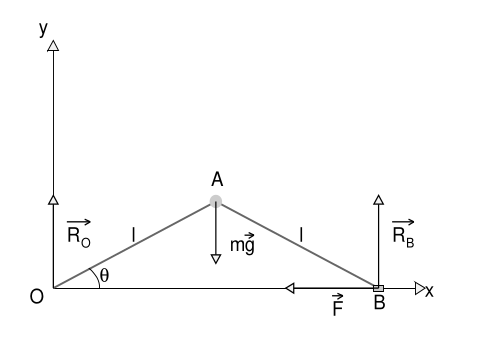
\includegraphics[width=0.7\textwidth]{images/mecanique_analytique/ma-001-000.png}
\caption{Système de treillis articulé : schéma.}
\end{figure}

\begin{figure}[H]
\centering
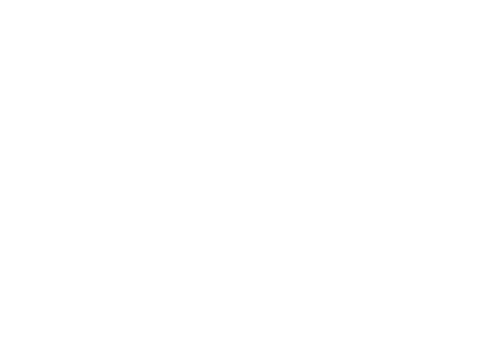
\includegraphics[width=0.7\textwidth]{images/mecanique_analytique/ma-001-001.png}
\caption{Forces et contraintes sur le treillis.}
\end{figure}

\begin{figure}[H]
\centering
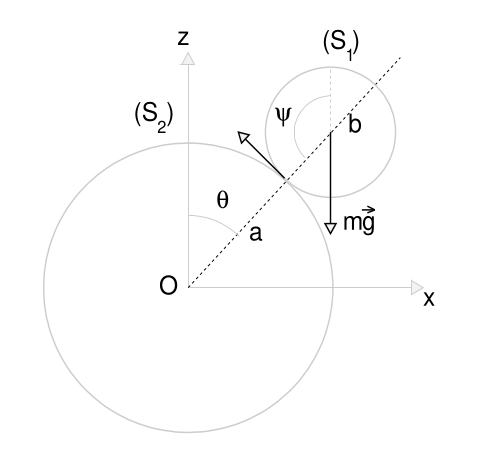
\includegraphics[width=0.7\textwidth]{images/mecanique_analytique/ma-003-002.png}
\caption{Roulement d'une sphère sur une autre.}
\end{figure}

\begin{figure}[H]
\centering
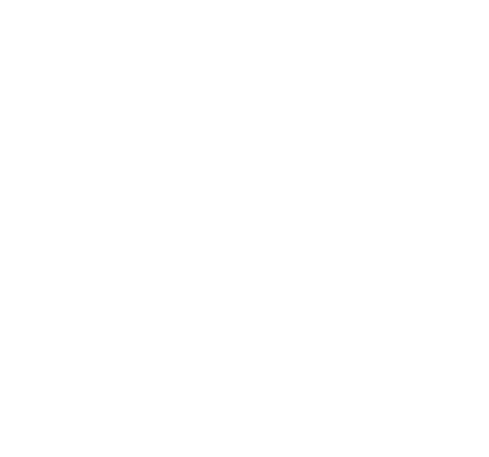
\includegraphics[width=0.7\textwidth]{images/mecanique_analytique/ma-003-003.png}
\caption{Électron en orbite : modèle planétaire.}
\end{figure}

\begin{figure}[H]
\centering
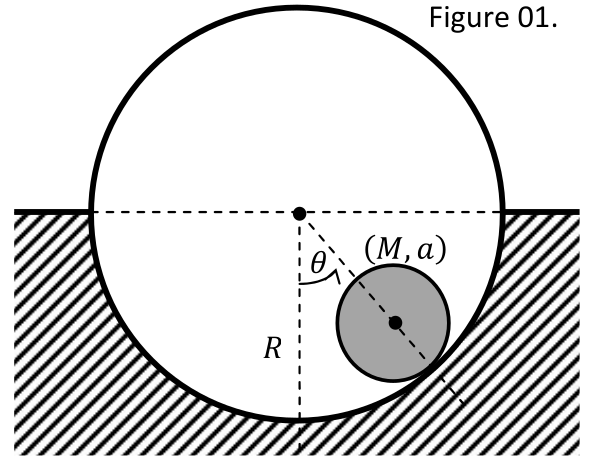
\includegraphics[width=0.7\textwidth]{images/mecanique_analytique/ma-011-004.png}
\caption{Pendule double : configuration.}
\end{figure}

\begin{figure}[H]
\centering
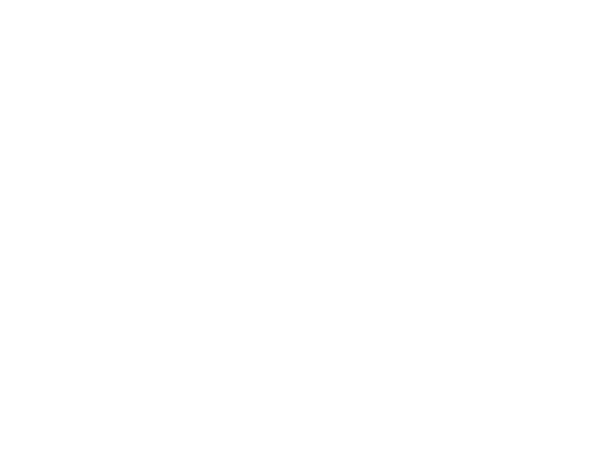
\includegraphics[width=0.7\textwidth]{images/mecanique_analytique/ma-011-005.png}
\caption{Modes normaux du pendule double.}
\end{figure}

\ifdefined\inMainDoc\else\end{document}\fi
